\chapter{Introdução}

\section{Elementos de um Circuito}

O livro de eletromagnetismo ideal é o do Griffiths 
\cite{GriffithsEletro}, o qual porém o 
do \cite[ver pag.10]{Adams1992,Niguem2013}.

Para analisarmos\cite{Campos2001,Heath1997,Dahlquist1974} um circuito 
precisamos conhecer os elementos que compõem o
mesmo. Vamos fazer um teste para citar \cite{Tort2001,Adams1992}.

Será feita uma simulação numérica\cite{Conte1980} dos resultados, e
para tal \ldots

\begin{equation}\label{eq:Sch} 
   i \hbar \dfrac{\partial \psi}{\partial t} = H \psi
\end{equation} 

\begin{postulado}
   Enuncia-se o postulado 1
\end{postulado}


\subsection{Resistor}

Um resistor (ôhmico, ou seja, aquele que obedece a lei de Ohm, $V=RI$)
é um elemento de circuito, representado pelo símbolo da figura 
\ref{fig:Resistor}. A lei de Ohm nos diz que: Quando por um resistor R passar
uma corrente I, haverá uma queda de potencial (no sentido da corrente:
$V=V_{1}-V_{2}$; $V_{1}>V_{2}$), através dos seus extremos 1 e 2, dada
por:
\begin{equation*}
V=RI
\end{equation*}

\begin{figure}[!h]
\begin{center}
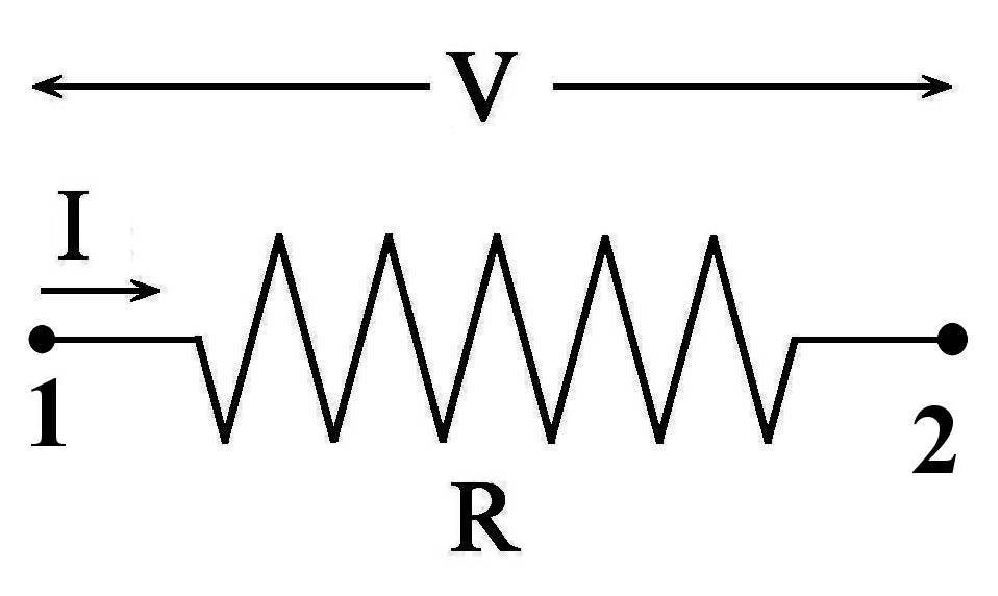
\includegraphics[width=0.70\linewidth]{Resistor_02.eps}
\end{center}
\caption{Resistor}
\label{fig:Resistor}
\end{figure}


Num resistor, há uma conversão de energia elétrica em energia
térmica, dada pelo efeito Joule. A potência dissipada pelo resistor
devido ao efeito Joule é dada por\cite{RLandau97,DeVries93}:
\begin{equation*}
P=RI^{2}=VI
\end{equation*}

\begin{equation}
M =
\begin{pmatrix}
1/a & x & x \\
-\cos\gamma/(a\sin\chi) & 2 & x \\
x & x & 3
\end{pmatrix}
\end{equation}

Na superfície da figura

\begin{figure}[!h]
\begin{center}
\includegraphics[width=0.70\linewidth,angle=-90]{Superficie.eps}
\end{center}
\caption{Teste 2}
\label{Resistor}
\end{figure}

Este gráfico foi feito no gnuplot usando
o modo pm3d. Na equação de Scrodinger (\ref{eq:Sch})
ou \eqref{eq:Sch}

\begin{comment}
Alguns dos comandos fornecidos pelo Scilab para gerenciar as funções
são apresentadas na tabela~\ref{tab:GenFunc} abaixo.
\begin{table}[!htb]
\begin{center}
\begin{tabular}{ A| m{10.0cm}}
\hline
\rowcolor[gray]{.8}
\textbf{Função}    &
\textbf{Significado} \\
\hline
\texttt{function}    & abre a definição de uma função \\
\texttt{endfunction} & fecha a definição de uma função \\
\hline
\texttt{argn}      & número de argumentos de entrada/saída de uma função\\
\texttt{varargin}  & variável com o número de argumentos da lista de entrada\\
\texttt{varargout} & variável com o número de argumentos da lista de saída\\
\hline
\texttt{fun2string}          & gera a definição ASCII de uma função do Scilab\\
\texttt{get\_function\_path} & obtém o caminho do arquivo fonte de uma biblioteca de funções\\
\texttt{getd}                & obtém todas as funções definidas em um diretório\\
\texttt{head\_comments}      & mostra o cabeçalho de comentários das funções do Scilab\\
\texttt{listfunctions}       & lista as propriedades de todas as funções no ambiente do Scilab\\
\texttt{macrovar}            & variáveis de uma função\\
\hline
\end{tabular}
\end{center}
\caption{Funções do Scilab para gerenciar funções.}
\label{tab:GenFunc}
\end{table}
\end{comment}

%\setlength\arrayrulewidth{2pt}\arrayrulecolor{blue}
%\setlength\doublerulesep{2pt}\doublerulesepcolor{blue}
\begin{table}
\begin{center}
\begin{tabular}{c | c | c}
0 & 2 & 3\\ \hline
\rowcolor{cinza}\multicolumn{1}{c}{5} & \multicolumn{1}{c}{5} & \multicolumn{1}{c}{5} \\
\hline
\rowcolor[gray]{.8} 1 & 1 & 1\\
4 & 6 & 8
\end{tabular}
\end{center}
\end{table}


\section{Introdução}

O Método das Diferenças Finitas (MDF) é um método geralmente
utilizado para resolver equações diferenciais. Inicialmente
discretizamos o espaço, e esta discretização poderá ser
uniforme ou não e posteriromente reescrevemos a equação\cite[ver pag. 34]{RLandau97}
diferencial em termos das diferenças. Nos casos que iremos estudar
agora, iremos considerar uma discretização não uniforme,
conforme a figura ~\ref{fig2} abaixo.

\begin{equation}
   x^2\Longleftrightarrow
\end{equation} 

\begin{figure}[htb]
\begin{center}
\setlength{\unitlength}{0.0040in}%
\begin{picture}(565,100)(15,450)
\thicklines
\put(150,480){\circle*{7}}
\put(170,480){\circle*{7}}
\put(190,480){\circle*{7}}
\put(415,480){\circle*{7}}
\put(435,480){\circle*{7}}
\put(455,480){\circle*{7}}
\put(-53,480){\line( 1, 0){185}}
\put(-60,480){\circle{15}}
%%\put(-60,490){\line( 0,-1){ 20}}
%%\put( 20,480){\line( 1, 0){100}}%%
%%\put( 20,490){\line( 0,-1){ 20}}
\put( 20,480){\circle*{15}}
\put( 20,470){\line( 0, 1){  0}}
%%\put(100,490){\line( 0,-1){ 20}}
\put(100,480){\circle*{15}}
\put(200,480){\line( 1, 0){200}}
\put(220,480){\circle*{15}}
\put(300,480){\circle*{15}}
\put(380,480){\circle*{15}}
\put(500,480){\circle*{15}}
\put(580,480){\circle*{15}}
%\put(220,490){\line( 0,-1){ 20}}
%\put(300,490){\line( 0,-1){ 20}}
%\put(380,490){\line( 0,-1){ 20}}
%\put(500,490){\line( 0,-1){ 20}}
%\put(580,490){\line( 0,-1){ 20}}
\put(480,480){\line( 1, 0){173}}
%\put(660,490){\line( 0,-1){ 20}}
\put(660,480){\circle{15}}
\put(225,500){\makebox(0,0)[lb]{\raisebox{0pt}[0pt][0pt]{ $\Delta x_{i-1}$}}}
\put(320,500){\makebox(0,0)[lb]{\raisebox{0pt}[0pt][0pt]{ $\Delta x_{i}$}}}
\put(-65,440){\makebox(0,0)[lb]{\raisebox{0pt}[0pt][0pt]{\large $0$}}}
\put( 15,440){\makebox(0,0)[lb]{\raisebox{0pt}[0pt][0pt]{\large $1$}}}
\put( 95,440){\makebox(0,0)[lb]{\raisebox{0pt}[0pt][0pt]{\large $2$}}}
\put(195,440){\makebox(0,0)[lb]{\raisebox{0pt}[0pt][0pt]{\large $i-1$}}}
\put(295,440){\makebox(0,0)[lb]{\raisebox{0pt}[0pt][0pt]{\large $i$}}}
\put(357,440){\makebox(0,0)[lb]{\raisebox{0pt}[0pt][0pt]{\large $i+1$}}}
\put(473,440){\makebox(0,0)[lb]{\raisebox{0pt}[0pt][0pt]{\large $n-1$}}}
\put(572,440){\makebox(0,0)[lb]{\raisebox{0pt}[0pt][0pt]{\large $n$}}}
\put(632,440){\makebox(0,0)[lb]{\raisebox{0pt}[0pt][0pt]{\large $n+1$}}}
%\put(247,490){\makebox(0,0)[lb]{\raisebox{0pt}[0pt][0pt]{\large $i-1$}}}
%\put(345,490){\makebox(0,0)[lb]{\raisebox{0pt}[0pt][0pt]{\large $i$}}}
\end{picture}
\end{center}
\vspace{-0.2cm}
\caption{Discretiza\c{c}\~{a}o da rede \label{fig2}}
\end{figure}%


Aqui iremos nos restringir a problemas em que temos equações
diferenciais de no máximo segunda ordem. Consideremos a expansão em 
série de Taylor da função $f(x)$ em torno do ponto $x_{i}$ (ver
figura ~\ref{fig2}). Na figura ~\ref{fig2} onde o índice $i$ indica um
ponto da rede discretizada, onde $f_{i}=f(x_{i})$ é o valor da 
função $f(x_{i})$ neste ponto e $\Delta _{i}=\Delta x_{i}=x_{i+1}-x_{i}$,
conforme mostra a figura~\ref{fig2}. Neste tipo de problema é muito
comum usarmos as seguintes condições de contorno: $f_{0}=f_{n+1}=0$,
$\Delta _{0}=\Delta _{1}$ e $\Delta _{n}=\Delta _{n-1}$.

\begin{align}
f(x+\Delta x_{i}) = & f(x) +\Delta x_{i}f^{\prime }(x) 
+\dfrac{\Delta x_{i}^{2}}{2!}f^{\prime \prime }(x) + \notag \\
& O(\Delta x_{i}^{3}) \label{df0}
\end{align}

\begin{align}
f(x+\Delta x_{i}) = & f(x)+\Delta x_{i}f^{\prime }(x)+
\dfrac{\Delta x_{i}^{2}}{2!}f^{\prime \prime }(x) + \notag \\ 
& O(\Delta x_{i}^{3})  \label{df1}
\end{align}

\begin{align}
f(x-\Delta x_{i-1}) = & f(x)-\Delta x_{i-1}f^{\prime }(x)+
\dfrac{\Delta x_{i-1}^{2}}{2!}f^{\prime \prime }(x) + \notag \\ 
& O(\Delta x_{i-1}^{3})  \label{df2}
\end{align}

\begin{align}
  & f(x+\Delta x_{i}) +f(x-\Delta x_{i-1}) \cong  2f(x) + \notag \\ 
  &\left( \Delta x_{i}-\Delta x_{i-1}\right) f^{\prime }(x) +
 \dfrac{(\Delta x_{i-1}^{2}+\Delta x_{i}^{2})}{2}f^{\prime \prime }(x)  
 \label{df3}
\end{align}

\begin{align}
  & f(x+\Delta x_{i}) - f(x-\Delta x_{i-1})  \cong  \notag \\ 
  & \left( \Delta x_{i-1} + \Delta x_{i} \right) f^{\prime }(x) -
 \dfrac{(\Delta x_{i-1}^{2}-\Delta x_{i}^{2})}{2} f^{\prime \prime }(x) \label{df4}
\end{align}
Podemos reescrever a eq. (\ref{df4}) como:

\begin{align}
f^{\prime }(x) & = \dfrac{f(x+\Delta x_{i})-f(x-\Delta x_{i-1})}{\Delta
x_{i-1}+\Delta x_{i}} - \notag \\ 
 & \dfrac{(\Delta x_{i}-\Delta x_{i-1})}{2}f^{\prime \prime }(x)  \label{df5}
\end{align}

Agora, substituindo a eq. (\ref{df5}) em (\ref{df3}), obtemos

% O estilos de referência se encontram no seguinte diretorio:
% /usr/share/texmf-texlive/bibtex/bst/

% O comando \nocite adiciona uma lista de referências sem que elas 
% necessitem de aparecer no texto.
\nocite{Franco2006,Heath1997,Davies-SciAm2006,Castro2001,Bolivar2001}

\nocite{AdvBashScr,BGB2008,Robbins2005,Neves2008,Jargas2008-Shell}
